\section{Конструкторский раздел}

\par В данном разделе углубленно описываются задействованные методы и алгоритмы. На их основе разрабатывается комбинированный метод прогнозирования временных рядов на фондовом рынке. Предложенная модель затем декомпозируется, выделяются ключевые этапы и особенности разработки, после приводится схема IDEF0.

\subsection{Авторегрессионные модели}

\subsubsection{ARIMA}

\par Autoregressive integrated moving average (ARIMA) ---  интегрированная модель авторегрессии —-- скользящего среднего классическая методология и модель анализа временных рядов. Идея данного алгоритма заключается в комбинировании процессов авторегрессии, процессов интегрирования и процессов скользящего среднего. Основной недостаток модели заключается в том, что ARIMA не предполагает включение дополнительных факторов, которые могут влиять на временной ряд. Модель базируется только на информации, содержащейся в предыстории прогнозируемого временного ряда.Одним из главных преимуществ ARIMA является способность моделировать интегрированные или разностно-стационарные временные ряды.

\par Самые распостраненные модели предсказаний для рынка акций основаны на моделях ARMA (Auto Regressive Moving Average) и ARIMA (Auto Regressive Integrated Moving Average). Модель ARMA (p,q) представляет из себя

\begin{equation}
	\label{eq:arima2}
    s_{t} = a_{0} + \sum_{i=1}^{p}a_{i}s_{t-i}+w_{t}+\sum_{i=1}^{q}b_{i}w_{t-i},
\end{equation}

где a и b - параметры, а w - шум.

\newpage

Эта модель может быть использована для стационарной последовательности \(s_{1:N}\), что соответственно означает

\begin{equation}
	\label{eq:arima3}
    E[s_{t}] = Constant
\end{equation}

\begin{equation}
    \label{eq:arima4}
    Cov(s_{t}, s_{t-k}) = Constant,
\end{equation}


где \(t = 1, 2, ..., N\) и \(k = 1, 2, ..., t.\)

В случае, когда последовательность не стационарна, ARIMA (p,q,d) используeт оператор разности временного ряда порядка d. В предсказаниях для рынка акций, разность первого порядка \(x_{1:N} = s_{1:N}\) (то есть \(x_{k} = s_{k}-s_{k-1}\)) обычно считается стационарной последовательностью.

Было проведено эмперическое исследование акций Банка Китая на китайском фондовом рынке. Цены акций фондового рынка являются публичными. Был выбран временной отрезок с 1 января 2007 по 31 марта 2022, где один день является единицей последовательности.

Тест ADF был выбран для тестирования стационарного условия временного ряда. Тестирование было проведено для первоначальной последовательности и для последовательности разности первого порядка. Результаты приведены в Таблице \ref{tab:ADF1} и \ref{tab:ADF2}. По результатам ADF теста можно заключить, что в случаях, когда p-значение больше 0.562 или критическое значение (1\%) больше -3.44, последовательность признается нестационарной, в то же время разница первого порядка последовательности --- стационарной. 
\newpage
Разница первого и второго порядка последовательности продемонстрированы на рисунках \ref{fig:first-order-diff} и \ref{fig:second-order-diff}.

\begin{table}[hbtp]
	\centering
	\caption{ADF тест для изначальной последовательности}
	\label{tab:ADF1}
	\resizebox{0.5\textwidth}{!}{%
		\begin{tabular}{|l|l|}
			\hline
			\textbf{Метрика} & \textbf{Значение}  \\ \hline
			Значение статистического теста               & -2.35539                 \\ \hline
			p-значение                 & 0.154726                 \\ \hline
			Кол-во использованных лагов               & 16                 \\ \hline
			Кол-во задействованных наблюдений             & 3484                 \\ \hline
			Критическое значение(1\%)            & -3.43223                 \\ \hline
			Критическое значение(5\%)            & -2.86237                 \\ \hline
			Критическое значение(10\%)            & -2.56721                 \\ \hline
		\end{tabular}%
	}
\end{table}

\begin{table}[hbtp]
	\centering
	\caption{ADF тест для разницы первого порядка}
	\label{tab:ADF2}
	\resizebox{0.5\textwidth}{!}{%
		\begin{tabular}{|l|l|}
			\hline
			\textbf{Метрика} & \textbf{Значение}  \\ \hline
			Значение статистического теста               & -14.7498               \\ \hline
			p-значение                 & 2.49575e-27                 \\ \hline
			Кол-во использованных лагов               & 15                 \\ \hline
			Кол-во задействованных наблюдений             & 3484                 \\ \hline
			Критическое значение(1\%)            & -3.43223                 \\ \hline
			Критическое значение(5\%)            & -2.86237                 \\ \hline
			Критическое значение(10\%)            & -2.56721                 \\ \hline
		\end{tabular}%
	}
\end{table}

\begin{figure}[hbtp]
  \centering
  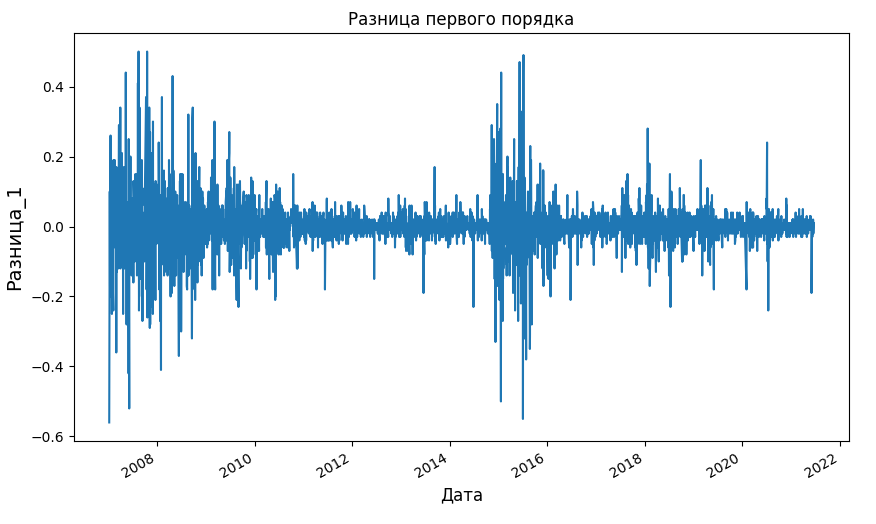
\includegraphics[width=0.85\textwidth]{img/first_order_diff.png}
  \caption{Разница первого порядка.}
  \label{fig:first-order-diff}
\end{figure}

\begin{figure}[hbtp]
  \centering
  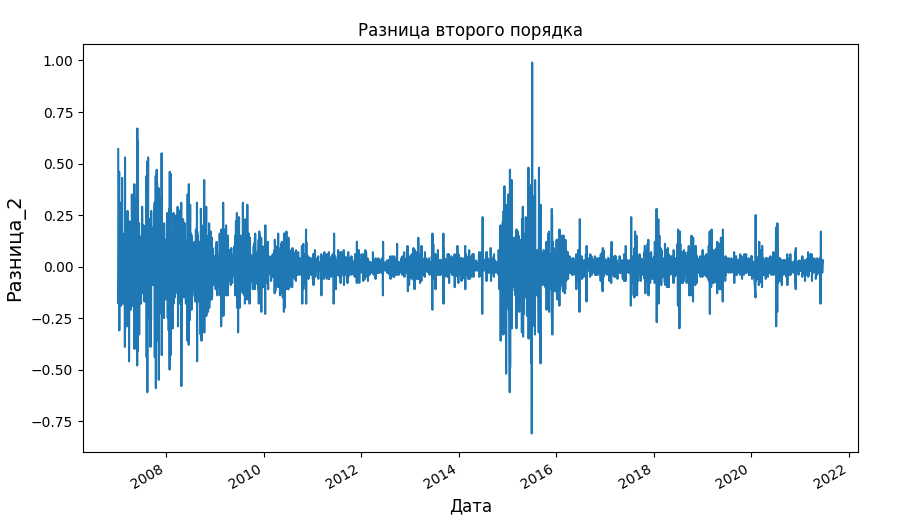
\includegraphics[width=0.85\textwidth]{img/second_order_diff.png}
  \caption{Разница второго порядка.}
  \label{fig:second-order-diff}
\end{figure}

\newpage

\subsection{Нейросетевые модели}

\subsubsection{Глубинное обучение на последовательности данных}

\par Как правило, для решения задач преобразования входной последовательности временных рядов в выходную последовательность той же или иной предметной области применяются соответствующие последовательные модели. В типичной нейронной сети с прямой связью (FFNN - feed-forward neural network), вывод текущего момента \(o_{t}\) определяется только входом текущего момента \(i_{t}\), как следствие возможности FFNN в моделирование временных рядов достаточно ограничены, что нельзя сказать о рекурентных нейронных сетях (RNN - recurrent neural network), которые создавались с  возможностью обработки длинных последовательных данных и решения задач с распределением контекста во времени.  В рекурентных нейронных сетях, используется задержка, чтобы сохранить текущее скрытое состояние последнего момента \(h_{t-1}\), затем, скрытое состояние текущего момента \(h_{t}\) определяется с помощью и \(h_{t-1}\), и \(i_{t}\), что продемонстрировано на рисунке под номером \ref{fig:RNN-unit}. 

\begin{figure}[hbtp]
  \centering
  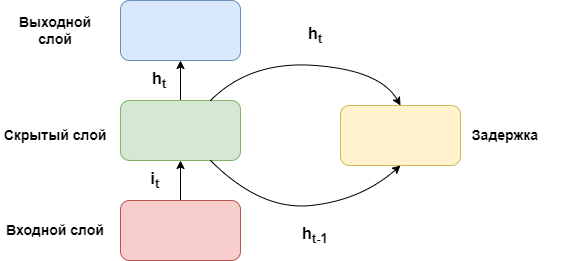
\includegraphics[width=0.6\textwidth]{img/RNN-unit.png}
  \caption{RNN блок.}
  \label{fig:RNN-unit}
\end{figure}

\par Модель обрабатывает по одному элементу последовательности на одном
временном шаге. После вычисления обновлённое состояние передается на
следующий шаг во времени, чтобы облегчить вычисление следующего
элемента. 

\par Тем не менее, исходя из следующей статьи \cite{OLD-LSTM}, можно утверждать, что высока вероятность того, что RNN может легко потерять долгосрочные зависимости, поэтому для решения проблемы забывания был разработан специализированный нейрон с усложненной внутренней структурой для запоминания долгосрочного контекста, называемого ячейкой long-short Term Memory (LSTM), которая схематично отображена на рисунке \ref{fig:lstm-scheme}.

\begin{figure}[hbtp]
  \centering
  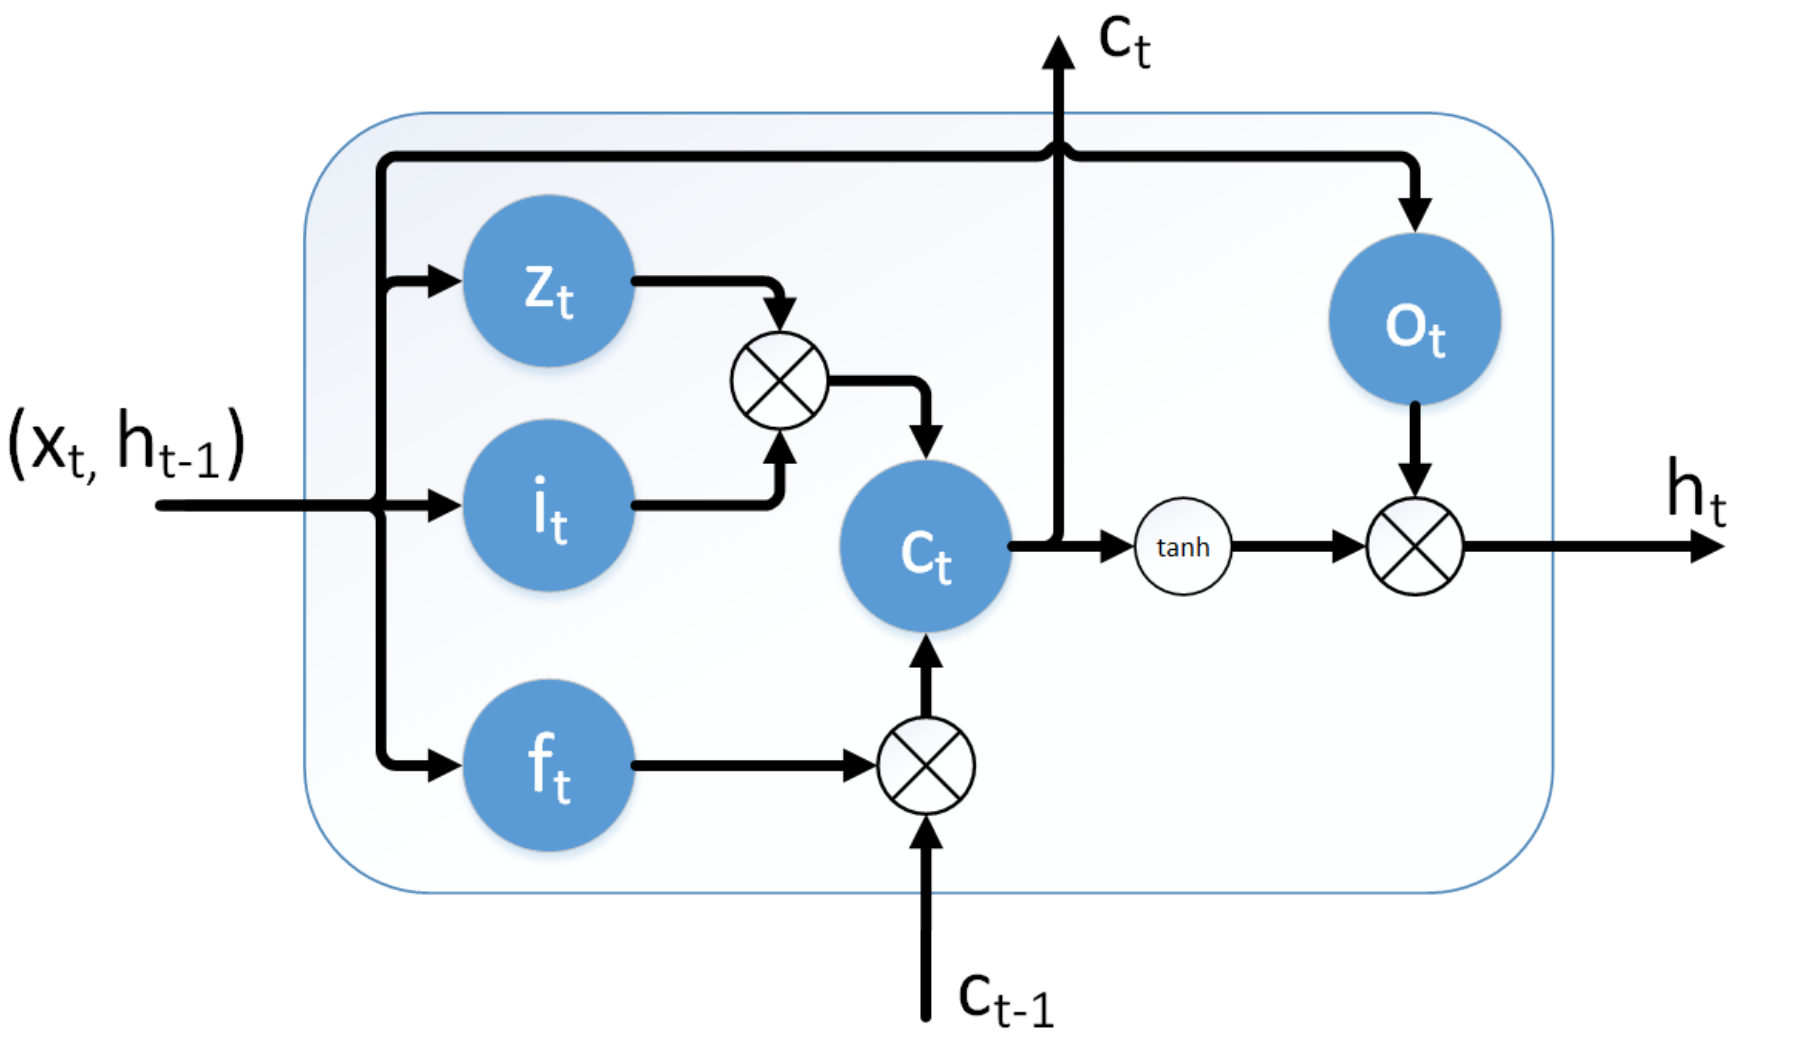
\includegraphics[width=0.8\textwidth]{img/lstm-scheme.png}
  \caption{LSTM блок.}
  \label{fig:lstm-scheme}
\end{figure}

\par Long-short term memory (LSTM) --— достаточно распространенная архитектура рекуррентной сети, идея этой архитектуры заключается в выделение ячейки памяти, ответственной за хранение информации, полученной в предыдущие моменты времени. Для управления этой ячейкой выделяются три шлюза:

\begin{itemize}[leftmargin=1.6\parindent]
    \item[---] \textit{Шлюз памяти}. Ответственен за сохранение или забывание предыдущего состояния ячейки.
	\item[---] \textit{Входной}. Контролирует поступление данных в память;
	\item[---] \textit{Исходящий}. Контролирует распространение данных из памяти;
\end{itemize}

\newpage

\par Функция ячейки памяти схожа с состояниями в детерминированном конченом автомате, однако в данном случае состояние «распределенное» и позволяет работать с бесконечным числом состояний. 

\begin{equation}
	\label{eq:lstm}
	\begin{tabular}{l}
        f_{t}=\sigma _{g}(W_{f}x_{t}+U_{f}h_{t-1}+b_{f})\\
        i_{t}=\sigma _{g}(W_{i}x_{t}+U_{i}h_{t-1}+b_{i})\\
        o_{t}=\sigma _{g}(W_{o}x_{t}+U_{o}h_{t-1}+b_{o})\\
        c_{t}=f_{t}\circ c_{t-1}+i_{t}\circ \sigma _{c}(W_{c}x_{t}+U_{c}h_{t-1}+b_{c})\\
        h_{t}=o_{t}\circ \sigma _{h}(c_{t})
    \end{tabular}
\end{equation}

где

\begin{itemize}[leftmargin=1.6\parindent]
    \item[] ${f_{t}}$ --- шлюз памяти; 
	\item[] ${i_{t}}$ --- входной шлюз;
	\item[] ${o_{t}}$ --- исходящий шлюз;
\end{itemize}

\par LSTM сети обучаются при помощи алгоритма обратного распространения ошибки сквозь время, идея которого состоит в разворачивании графа вычислений во времени. Из LSTM сетей можно выстраивать многослойные нейронные сети, передавая выходную последовательность очередного слоя на вход
следующему.

\par Sequence-to-sequence (seq2seq) модель использует автоматический кодировщик (модель, состоящая из двух рекуррентных сетей: кодировщика и декодировщика) для анализа последовательных данных, тем самым улучшая возможность LSTM моделей обучаться скрытой информации, не смотря на зашумленность данных. Кодировщик строит представление входной последовательности временных рядов (обычно скрытое состояние в последний момент последовательности \(h_{N}\)). Далее полученное представление (последние выход и значение ячейки сети) копируются в декодировщик. По полученному представлению декодировщик пытается восстановить целевую последовательность. 

\par Во время предсказания требуется найти наиболее вероятное продолжение последовательности временных рядов с точки зрения модели. Сделать это напрямую невозможно, так как модель позволяет вычислять только наилучшую последовательность при фиксированние предыдущих. Компромиссным решением между жадным выбором последовательностей и полным перебором является лучевой поиск. 

\par Лучевой поиск и алгоритм Витерби в скрытой цепи Маркова (HMM - Hidden Markov Model) оба основаны на динамическом программировании. Поиск оптимальной оценки значения текущего состояния, используя наблюдения и предыдущее состояние, называется декодированием (или интерференцией) в HMM. Высчитывая \(p(x_{k}|y_{1:k})\) и \(p(x_{k}|y_{1:N})\), соответственно, эквивалентно алгоритму двунаправленности в HMM. Оптимальная двусторонняя оценка может быть получена через распределение \(x_{k}\). 

\subsubsection{Механизм внимания}

Люди, в целом, обращают внимание на заметную, выделяющуюся из общего контекста информацию. В сверточных нейронных сетях, механизм внимания --- это метод, основанный на когнитивном восприятии человека. Для ввода \(X = (x_{1}, x_{2}, ..., x_{N})\), дан вектор запроса \(q\), индекс выбранной информации вниманием \(z = 1, 2, ..., N\), то распределение внимания --- это

\begin{equation}
    \label{eq:alpha-i}
    \alpha_{i} = p(z=i|X, q) = \frac{exp(s(x_{i}, q))}{\sum_{j=i}^{N}exp(s(x_{j}, q))}, 
\end{equation}

то есть,

\begin{equation}
    \label{eq:alpha-i-softmax}
    \alpha_{i} = softmax(s(x_{i}, q)), 
\end{equation}

где

\begin{equation}
    \label{eq:s-xi-q}
    s(x_{i}, q) = \frac{x_{i}^{T}q}{\sqrt{d}}
\end{equation}

\newpage

Есть количество очков внимания через маштабированное скалярное произведение, а \(d\) --- это измерение вводных данных. Предположим, что ввод - это пары ключ-значение \((K,V) = [(k_{1}, v_{1}), ..., (k_{N}, v_{N})] \), для данного значения \(q\), то функция внимания --- это

\begin{equation}
    \label{eq:att-k-v}
    att((K,V),q) = \sum_{i=1}^{N}\alpha_{i}v_{i} = \sum_{i=1}^{N}\frac{exp(s(k_{i},q))}{\sum_{j}exp(s(k_{i},q))}v_{i}
\end{equation}

Механизм множества внимания обычно используется через множество запросов \(Q = [q_{1}, ..., q_{M}]\) для вычисления функции внимания:

\begin{equation}
    \label{eq:att-k-v-q}
    att((K,V),Q) = (att((K,V),q_{1})\left \| ... \right \|att((K,V),q_{M}))
\end{equation}

Здесь, оператор || обозначает оператор объединения. Это и есть, так называемый, механизм множества внимания.

Механизм внимания может быть использован для генерации различных весов на основе данных. \(Q, K, V\) получены через линейную трансформацию \(X\), а \(W_{Q}, W_{K}, W_{V}\) могут быть динамически скорректированы. 

\begin{equation}
    \label{eq:q}
    Q = W_{Q}X, Q = W_{K}X, Q = W_{V}X
\end{equation}

Это так называемое само-внимание. Похожим образом, вывод - это

\begin{equation}
    \label{eq:h-i}
    h_{i} = att((K, V), q_{i})
\end{equation}

Используя маштабированное скалярное произведение, мы получаем

\begin{equation}
    \label{eq:h-v-softmax}
    H=V softmax( K^{T} Q\frac{1}{\sqrt{d}} )
\end{equation}

\subsection{Предложенная модель}

\par Реализация модели построена на комбинирование классических методов ARIMA, ACNN, BiLSTM и является гибридной моделью глубокого обучения для предсказания курса акций. Основное отличие разработанной модели от традиционных аналогов --- это интеграция модели исследования временных рядов ARIMA и нейронных сетей в нелинейной зависимости, которая позволяет объединить преимущества двух классических моделей с целью повышения точности предсказаний. Общая схема предложенной модели представлена на рисунке \ref{fig:model-scheme}.

\begin{figure}[hbtp]
  \centering
  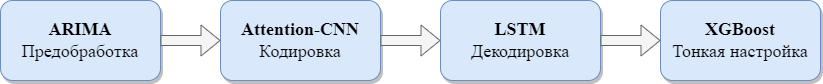
\includegraphics[width=0.9\textwidth]{img/model.png}
  \caption{Блок-схема разработанной комбинированной модели.}
  \label{fig:model-scheme}
\end{figure}

\par Первоначально курс акций проходит обработку через ARIMA, затем сформированная последовательность задействуется в нейронных сетях. Основная идея на этом этапе заключается в том, что изначальные данные фондового рынка помещенные в модель ARIMA стационарными взятием разностей некоторого порядка от исходного временного ряда (так называемые интегрированные или разностно-стационарные временные ряды), позволяют получить новый ряд, отображающим с большей эффективностью характеристику курса акций.

\par Затем архитектура глубокого обучения формируется в рамках предобучения-дообучения с применением фрэймворков.
Предобучающая модель представляет собой CNN-LSTM модель на основе механизма внимания с использованием подхода машинного обучения seq2seq, где модель CNN на основе механизма внимания является кодировщиком, а двунаправленная модель LSTM декодировщиком соответственно. Предназначения используемых моделей можно представить следующим образом:

\begin{itemize}[leftmargin=1.6\parindent]
    \item[---] CNN модель на основе механизма внимания извлекает глубинные характеристики временного ряда;
	\item[---] LSTM модель добывает долгосрочные характеристики временного ряда;
	\item[---] XGBoost модель используется для тонкой настройки, позволяя полностью получить информацию о фондовом рынке за несколько периодов.
\end{itemize}

\par Также важно отметить, что применение подхода машинного обучения \\
seq2seq позволяет подавить влияние шума при помощи используемой архитектуры кодировщик-декодировщик.
На основе глубокого обучения скрытая информация о состоянии отображается более эффективно, пока модель
не будет удовлетворять предположениям о линейных свойствах цены акции. 
В целом, слои кодировщик-декодировщик отображают зависимость между нынешней и предыдущей последовательностью, а также между нынешней последовательностью и эмбеддингами.

\par Основным аргументом в пользу использования модели CNN на основе механизма внимания, в сочетание с моделью LSTM является тот факт, что CNN модель способна выявлять глобальные и локальные зависимости, которые не всегда улавливаются LSTM моделью. Причина описанного ранее явления кроется в том, что используемая модель CNN совмещается в себе, как и слои свертки, так и слои множенственного внимания. В итоге совмещение LSTM модели с CNN моделью повышает, как и структурные преимущества, так и способности моделировния временных рядов. 

\par После декодерирования выходные данные поподают в XGBoost регрессор для более тщательного извлечения характеристик и тонкой настройки. 
Как модель для тонкой настройки XGBoost обладает рядом внушительных преимуществ, которыми являются расширяемость и гибкость. Данная модель интегрирует несколько различных модельных деревьев для получения более эффективной модели обучения, как итого XGBoost модель повышает конечные прогностические и обобщающие способности модели.

\newpage

\subsection{IDEF0-диаграмма}

\par На рисунках \ref{fig:idef0} и \ref{fig:idef0a1} представлена диаграмма IDEF0 комбинированного метода прогнозирования временных рядов на фондовом рынке.

\begin{figure}[hbtp]
  \centering
  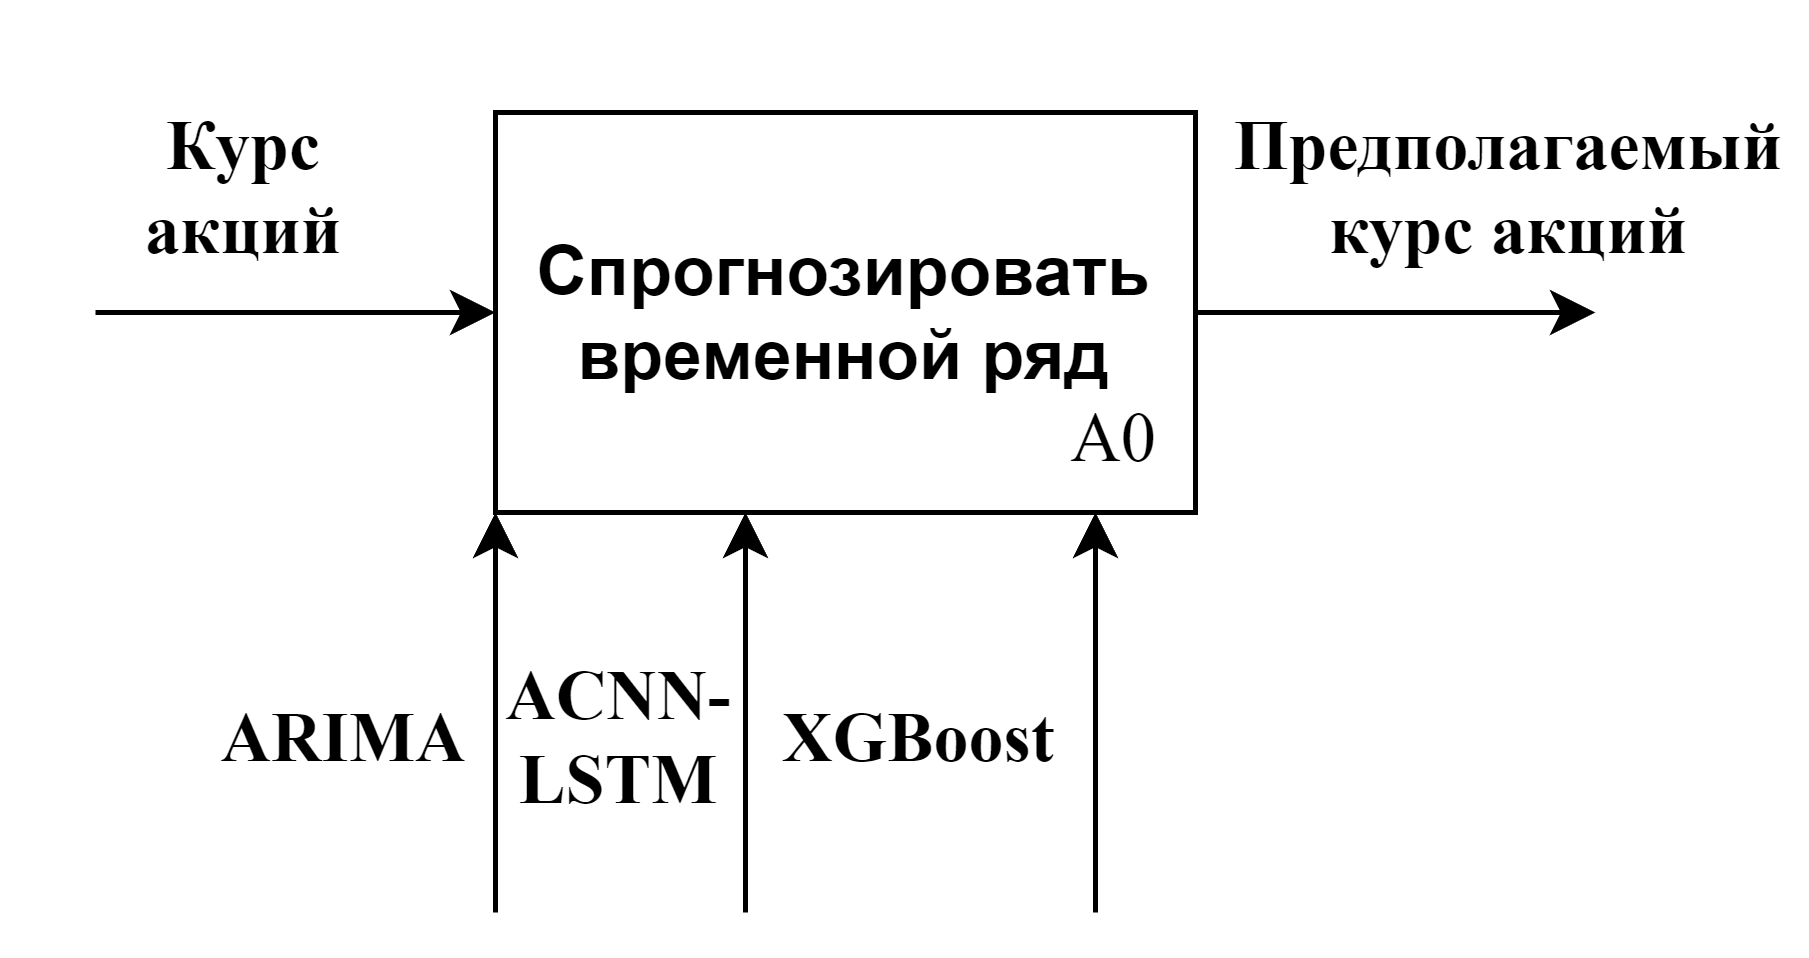
\includegraphics[width=0.8\textwidth]{img/IDEF0.png}
  \caption{Функциональная модель метода в виде IDEF0 — диаграммы уровня A0.}
  \label{fig:idef0}
\end{figure}


\begin{figure}[hbtp]
  \centering
  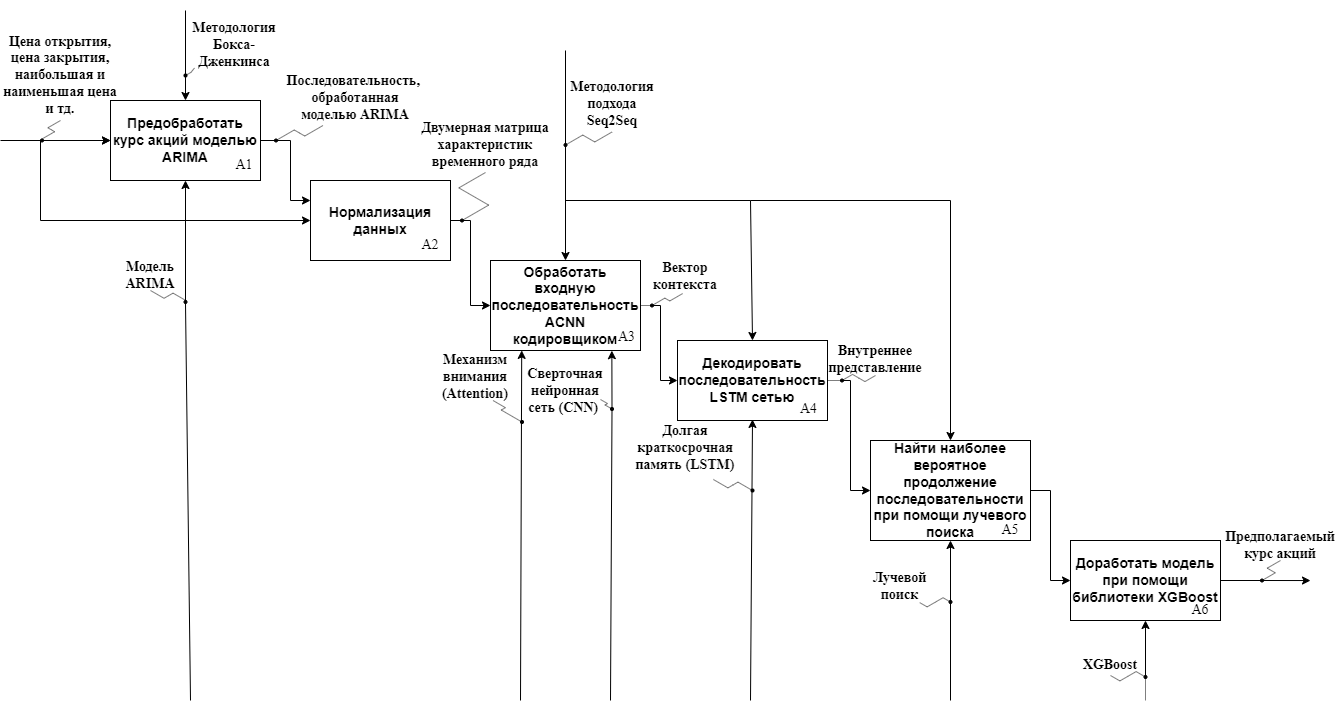
\includegraphics[width=0.8\textwidth]{img/IDEF0A1.png}
  \caption{Функциональная модель метода в виде IDEF0 — диаграммы уровня A1-A6.}
  \label{fig:idef0a1}
\end{figure}


\subsection{Выводы из конструкторского раздела}
\par В рамках данного раздела были углубленно изложены задействованные методы и алгоритмы, на их основе разработан и описан комбинированный метод, который затем был декомпозицирован. Основой разработанного комбинированного метода выступили такие классические модели, как ARIMA, ACNN, BiLSTM, исходя из предположения, что их интеграция в нелинейной зависимости способна улучшить эффективность предсказания временных рядов.
\pagebreak 